\chapter{Rezultate}
\section{Optim fix}
Pentru un nivel simplu, cu un singur obstacol, in care atat obstacolul cat si tinta sunt statice, algoritmul genetic reuseste sa convearga la tinta relativ rapid. Urmatoarele doua teste ruleaza cu o populatie $\lambda = 100$ , un numar maxim de iteratii $k = 100$ unde o rata de mutatie de 10$\%$ a genomului poate avea loc uniform in populatie cu o probabilitate  $p \in \{0.05, 0.1\}$, iar metoda de crossover este Single Point Crossover.
\begin{center}
    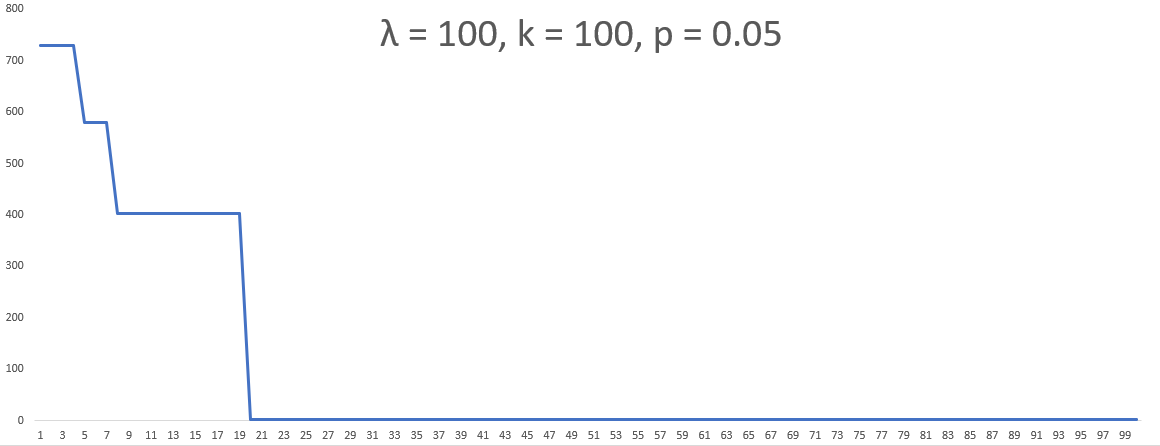
\includegraphics[width=0.7\textwidth]{results/p100i100m10p005.png}
    \linebreak
    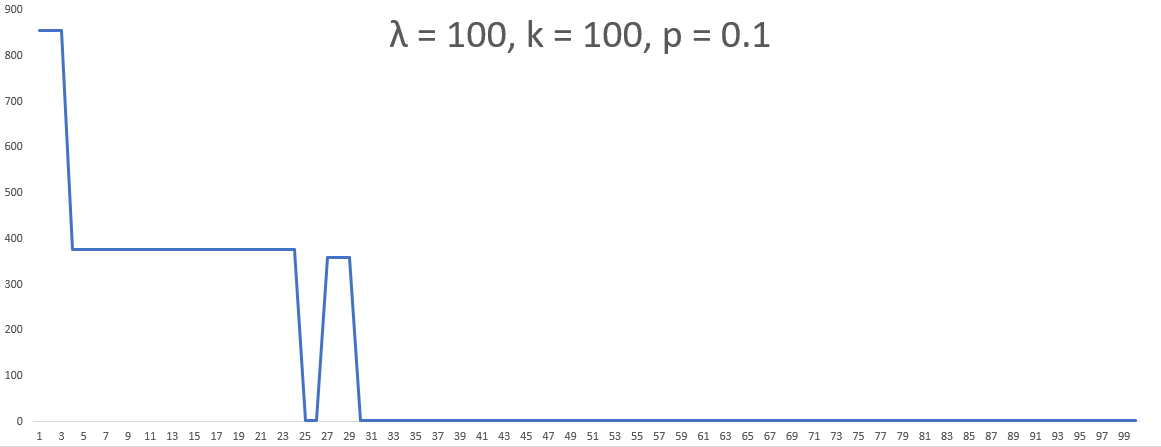
\includegraphics[width=0.7\textwidth]{results/p100i100m10p01.png}
\end{center}

Pentru o populatie $ \lambda=100 $ si un nivel relativ usor, algoritmul genetic converge in cateva zeci de generatii, tipul de crossover sau probabilitatea mutatiei avand impact minimal.

Odata cu scaderea populatiei maxime, algoritmul genetic are sanse tot mai mari de a se bloca intr-un optim local:
\begin{center}
    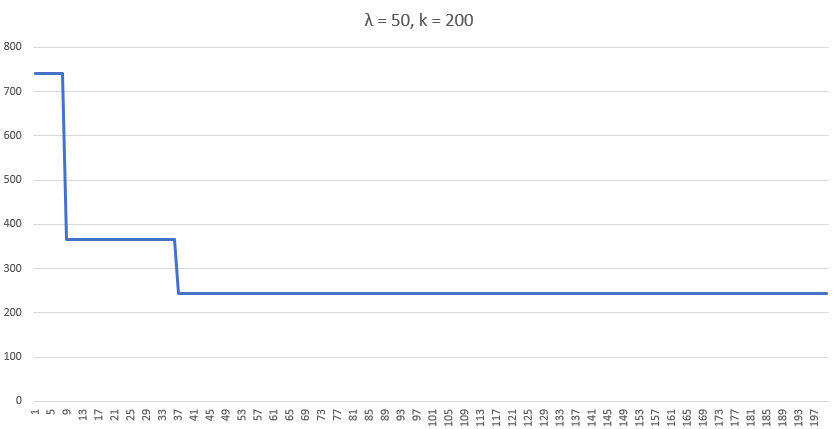
\includegraphics[width=0.7\textwidth]{results/p50k200localoptim.png}
\end{center}

Avand $2^{21}$ combinatii posibile pentru un cromozom de lungime 21, fara o generatie initiala bogata, algoritmul poate ajunge intr-un optim local. Vizualizand populatia, invidivii ajung langa tinta dar nu o ating sau raman sub ea.

O solutie pentru blocarea intr-un optim local, este marirea ratei de mutatie, a iteratiilor sau a modalitatilor de selectie. Dupa marirea parametrilor de mutatie la $p=0.15$, a ratei de mutatie a genomului la $15\%$ si a numarului de iteratii pana la 1500, algoritmul genetic reuseste sa iasa ajunga in optimul global dupa 1200 de iteratii:

\begin{center}
    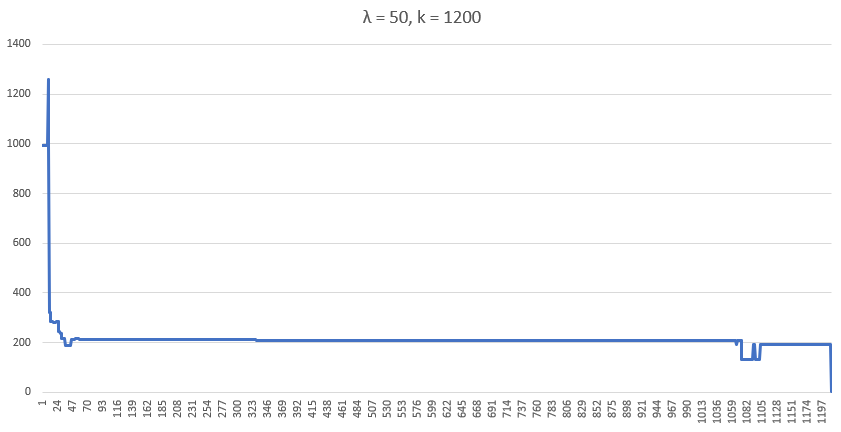
\includegraphics[width=0.7\textwidth]{results/p50k1200localoptimdefeat.png}
\end{center}

\section{Optim dinamic}

Pentru a obtine o problema de optim dinamic in mediul fizic, inducem o rotatie obstacolelor, deci acum au "ferestre" in care se pot trece prin ele iar tinta se va roti si ea , nu mai putand fi atinsa in aceleasi locuri la orice moment de timp. Luand initial o populatie $\lambda = 100$ si $k=200$ iteratii, algoritmul genetic reuseste sa convearga in sub 100 de generatii:

\begin{center}
    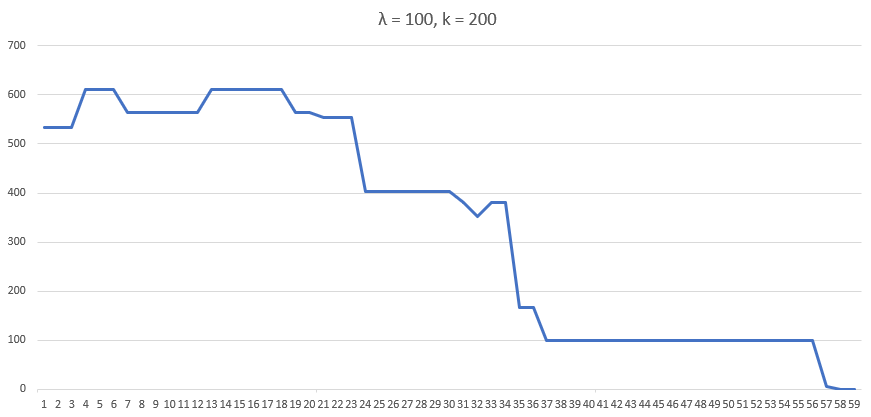
\includegraphics[width=0.7\textwidth]{results/optimdinamicp100k200.png}
\end{center}

Adaugand o translatie pe axa y a obstacolelor si folosind aceeasi configuratie pentru populatia initiala si iteratii, algoritmul genetic gaseste o traiectorie care trece pe sub obstacol imediat dupa ce acesta se ridica.

\begin{center}
    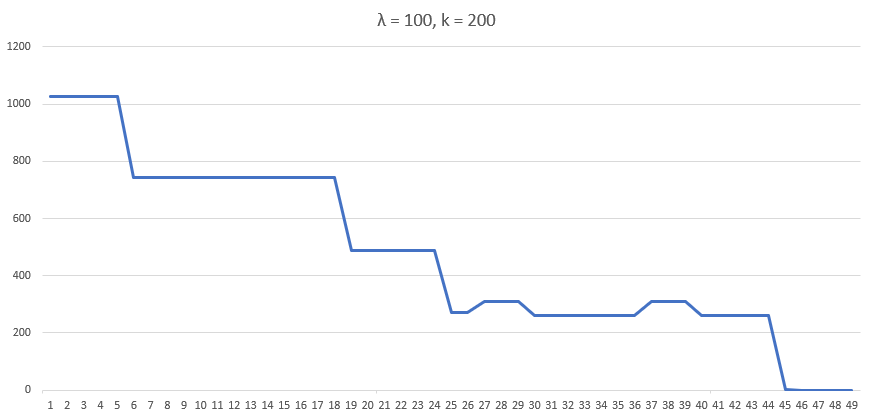
\includegraphics[width=0.7\textwidth]{results/optimdinamicp100k200moving.png}
\end{center}

Se observa convergenta rapida pentru $\lambda = 100$ atat in optime dinamice cat si fixe. 